\documentclass[11,]{article}
\usepackage{lmodern}
\usepackage{amssymb,amsmath}
\usepackage{ifxetex,ifluatex}
\usepackage{fixltx2e} % provides \textsubscript
\ifnum 0\ifxetex 1\fi\ifluatex 1\fi=0 % if pdftex
  \usepackage[T1]{fontenc}
  \usepackage[utf8]{inputenc}
\else % if luatex or xelatex
  \ifxetex
    \usepackage{mathspec}
  \else
    \usepackage{fontspec}
  \fi
  \defaultfontfeatures{Ligatures=TeX,Scale=MatchLowercase}
\fi
% use upquote if available, for straight quotes in verbatim environments
\IfFileExists{upquote.sty}{\usepackage{upquote}}{}
% use microtype if available
\IfFileExists{microtype.sty}{%
\usepackage{microtype}
\UseMicrotypeSet[protrusion]{basicmath} % disable protrusion for tt fonts
}{}
\usepackage[margin=1in]{geometry}
\usepackage{hyperref}
\PassOptionsToPackage{usenames,dvipsnames}{color} % color is loaded by hyperref
\hypersetup{unicode=true,
            colorlinks=true,
            linkcolor=Maroon,
            citecolor=Blue,
            urlcolor=blue,
            breaklinks=true}
\urlstyle{same}  % don't use monospace font for urls
\usepackage{longtable,booktabs}
\usepackage{graphicx,grffile}
\makeatletter
\def\maxwidth{\ifdim\Gin@nat@width>\linewidth\linewidth\else\Gin@nat@width\fi}
\def\maxheight{\ifdim\Gin@nat@height>\textheight\textheight\else\Gin@nat@height\fi}
\makeatother
% Scale images if necessary, so that they will not overflow the page
% margins by default, and it is still possible to overwrite the defaults
% using explicit options in \includegraphics[width, height, ...]{}
\setkeys{Gin}{width=\maxwidth,height=\maxheight,keepaspectratio}
\IfFileExists{parskip.sty}{%
\usepackage{parskip}
}{% else
\setlength{\parindent}{0pt}
\setlength{\parskip}{6pt plus 2pt minus 1pt}
}
\setlength{\emergencystretch}{3em}  % prevent overfull lines
\providecommand{\tightlist}{%
  \setlength{\itemsep}{0pt}\setlength{\parskip}{0pt}}
\setcounter{secnumdepth}{5}
% Redefines (sub)paragraphs to behave more like sections
\ifx\paragraph\undefined\else
\let\oldparagraph\paragraph
\renewcommand{\paragraph}[1]{\oldparagraph{#1}\mbox{}}
\fi
\ifx\subparagraph\undefined\else
\let\oldsubparagraph\subparagraph
\renewcommand{\subparagraph}[1]{\oldsubparagraph{#1}\mbox{}}
\fi

%%% Use protect on footnotes to avoid problems with footnotes in titles
\let\rmarkdownfootnote\footnote%
\def\footnote{\protect\rmarkdownfootnote}

%%% Change title format to be more compact
\usepackage{titling}

% Create subtitle command for use in maketitle
\providecommand{\subtitle}[1]{
  \posttitle{
    \begin{center}\large#1\end{center}
    }
}

\setlength{\droptitle}{-2em}

  \title{}
    \pretitle{\vspace{\droptitle}}
  \posttitle{}
    \author{}
    \preauthor{}\postauthor{}
    \date{}
    \predate{}\postdate{}
  
\usepackage{setspace}
\usepackage{hyperref}
\usepackage{graphicx}

\begin{document}

%%% .rmd + .sty setup borrowed from: https://github.com/oganm/ThesisProposal

\onehalfspacing
\pagenumbering{gobble}

%\begin{titlepage}
\begin{center}
\huge{\textbf{New Tools to Interactively Explore Sensitivity of Structure in Low-dimensional Projections of Data}}\\
\vspace*{1\baselineskip}
\Large{\textbf{Mid-candidature review --- 25 February, 2020}}\\
%\vspace*{1\baselineskip}
\LARGE{Nicholas Spyrison, B.Sc}\\
\vspace*{1\baselineskip}

\LARGE{Monash University}\\
\Large{Faculty of Information Technology}\\
\vspace*{1\baselineskip}

\includegraphics[height = 3.5cm]{./figures/crest.jpg}\\
\vspace*{1\baselineskip}

\Large{\textbf{Thesis Supervisors}}\\
Prof. Kimbal Marriott\\
Prof. Dianne Cook\\
\vspace*{1\baselineskip}
\Large{\textbf{Committee Members}}\\
Dr. Maxime Cordiel\\
Dr. Shirui Pan\\
\vspace*{1\baselineskip}
\Large{\textbf{Chair}}\\
Assoc. Prof. Bernhard Jenny\\
\end{center}
% \end{titlepage}

\doublespacing

%\hypersetup{linkcolor = blue}
\newpage
\pagenumbering{roman}
\addcontentsline{toc}{section}{\contentsname}

\newpage

%% list of figures have to be added manually to table of contents
% \listoffigures 
% 
% \newpage
% \listoftables

\doublespacing

\newpage
\pagenumbering{arabic}
\hypersetup{linkcolor = blue}

{
\hypersetup{linkcolor=black}
\setcounter{tocdepth}{2}
\tableofcontents
}
\hypertarget{sec:intro}{%
\section{Introduction}\label{sec:intro}}

\hypertarget{motivation}{%
\subsection{Motivation}\label{motivation}}

The term exploratory data analysis (EDA) was coined by Tukey (1977), who leaves it as an intentionally broad term that encompasses the initial summarization and visualization of a data set. This is a critical first step of checking for realistic values and validating model assumptions. It may be tempting to review a series of summary statistics to check model assumptions. However, there are known datasets where the same summary statistics miss glaringly obvious visual patterns (Anscombe 1973; Matejka and Fitzmaurice 2017). It is strikingly simple to look at the wrong, or incomplete set of statistics needed to validate assumptions. Data visualization is fast, versatile, and robust relative to the alternative of numeric statistical summarization. Data visualization does and must remain a primary component of data analysis and model validation.

Data and models are typically \textbf{high-dimensional}, with many variables, and possibly many model parameters. Conventionally, \(n\) is used for the number of sample observations, and \(p\) is used for the number of variables. Developing new methods to visualize high dimensions has been a pursuit of statisticians, computer scientists and visualization researchers for decades. While automated analysis is the norm, there remains some benefit of user interaction to help the analyst understand results, and determine the importance of components in a model. An interplay between automated and human-centered control is useful. As technology changes, new approaches to user interaction emerge, and exploring these technologies provides a challenge to researchers.

Linear projections are commonly used to reduce the dimensionality. A \textbf{linear projection} is the linear transformation of the \(p\)-dimensional space into a low-(\(d-\))dimensional space, by matrix multiplication of the data with an orthonormal \(p\times d\) basis. An orthonormal basis has columns that are orthogonal to each other, and of length 1.

Good linear projections are often found with an automated procedure, like principal component analysis (PCA; Pearson 1901) or projection pursuit (Kruskal (1969)). These reduce the dimensionality and reveal something interesting about the data. Figure \ref{fig:basis} shows a \(d=2\) dimensional projection of \(6D\) data, revealing clustering of labelled groups. The basis that produced this projection is

\begin{equation*}
\left[ \begin{array}{rr}
 0.39 &  0.08 \\
 0.11 &  0.21 \\
 0.18 &  0.33 \\
 0.45 & -0.01 \\
 0.41 & -0.11 \\
 0.09 &  0.32 \\
 0.15 &  0.21 \\
 0.60 & -0.18 \\
 0.02 &  0.34 \\
 0.15 &  0.14 \\
-0.09 &  0.51 \\
 0.07 &  0.37 \\
-0.06 &  0.34 \\
\end{array} \right]
\end{equation*}

\begin{figure}[h]

{\centering 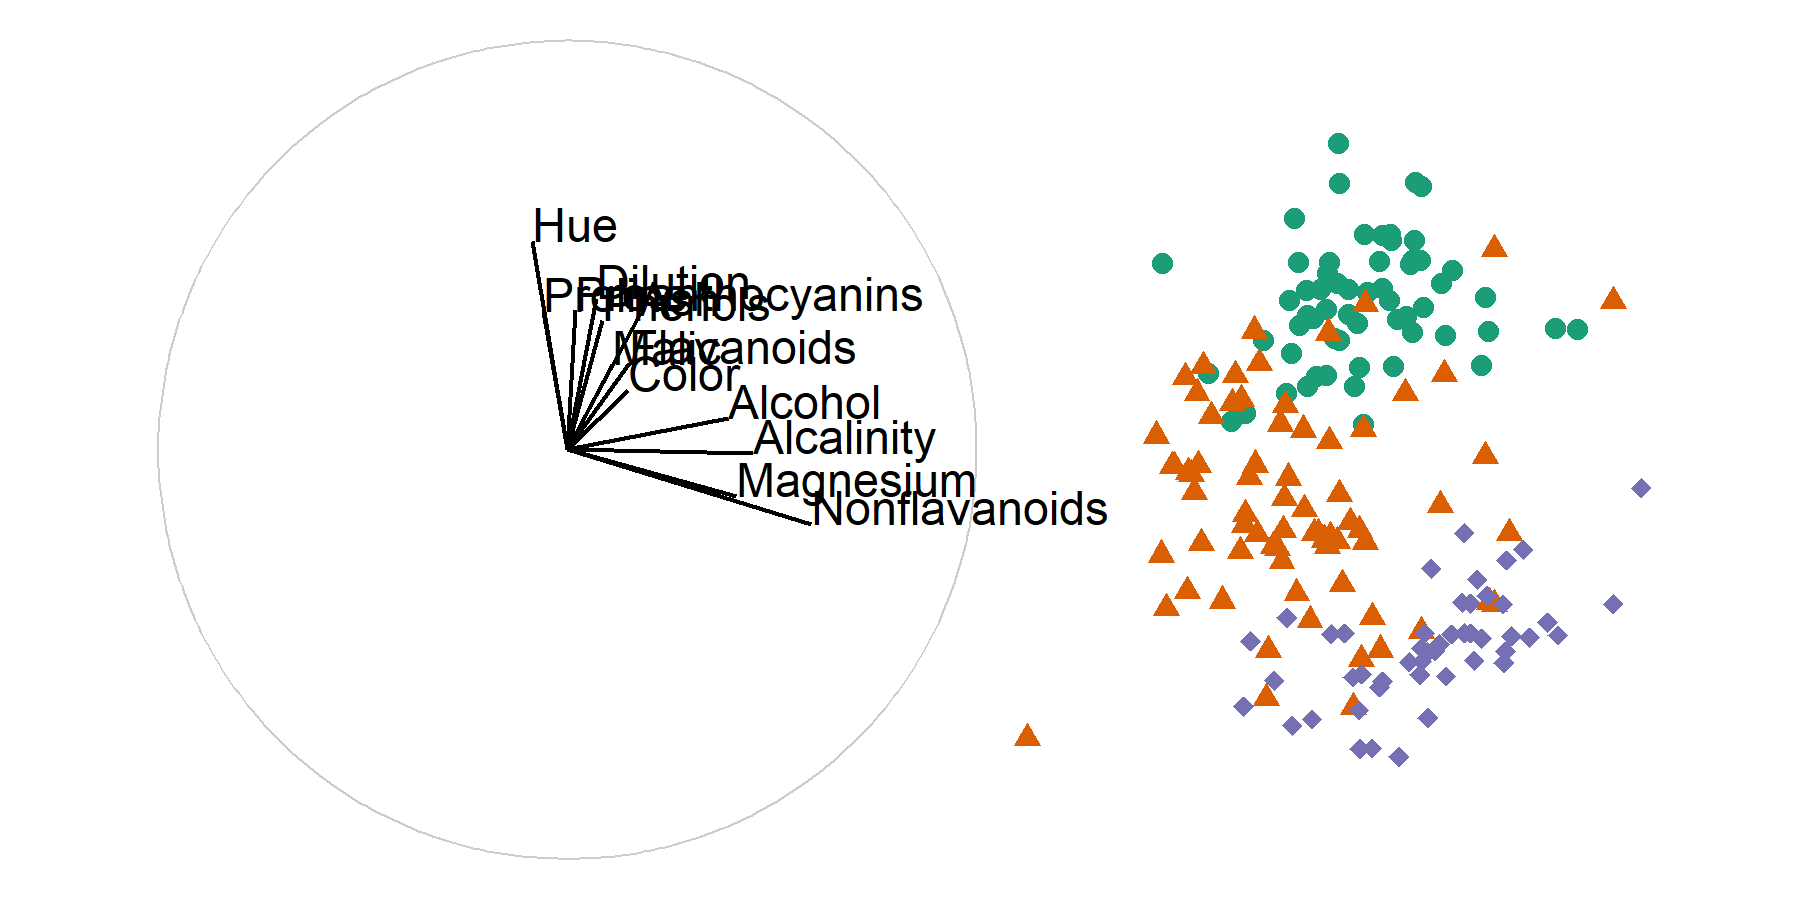
\includegraphics[width=1\linewidth,]{./figures/basisWINE} 

}

\caption{FIXME CAP NEEDED.}\label{fig:basis}
\end{figure}

Projection + Data (original)

Projection + Data (one variable rotated out, with no effect to structure)

Projection + Data (one variable rotated out, with structure lost)

Figure \ref{fig:basisStructure} shows how \textbf{sensitivity of structure} in a projection can depend on variables contributing to the projection. When variable Phenols is rotated out, there is no change to the structure, clusters are still visible. This says that the structure \emph{is NOT sensitive} to variable Phenols When variable Alcalinity is rotated out, there is change to the structure, clusters are less visible. This says that the structure \emph{is sensitive} to variable Alcalinity

Exploring the sensitivity of structure in a projection to the contributions of particular variables requires \textbf{geodsic interpolation} to remove the variable from (or into) the projection plane. Geodesic interpolation is effectively a rotation, it maintains orthonormality of all new data projections, and any intermediate projections. Geodesic interpolation is used in tour methods (FIXME: REF), including the \textbf{grand tour} which shows (automated) movies of low-dmensional projections of high-dimensional spaces. The \texttt{tourr} package (Wickham et al. 2011) in R provides a range of automated tours.

Sensitivity analysis is ideally achieved with \textbf{user-controlled steering} where the human controls the rotation of a variable into and out of a projection. This will enable various intermediate states to be shown to better understand the effect of single variables.

\begin{figure}[h]

{\centering 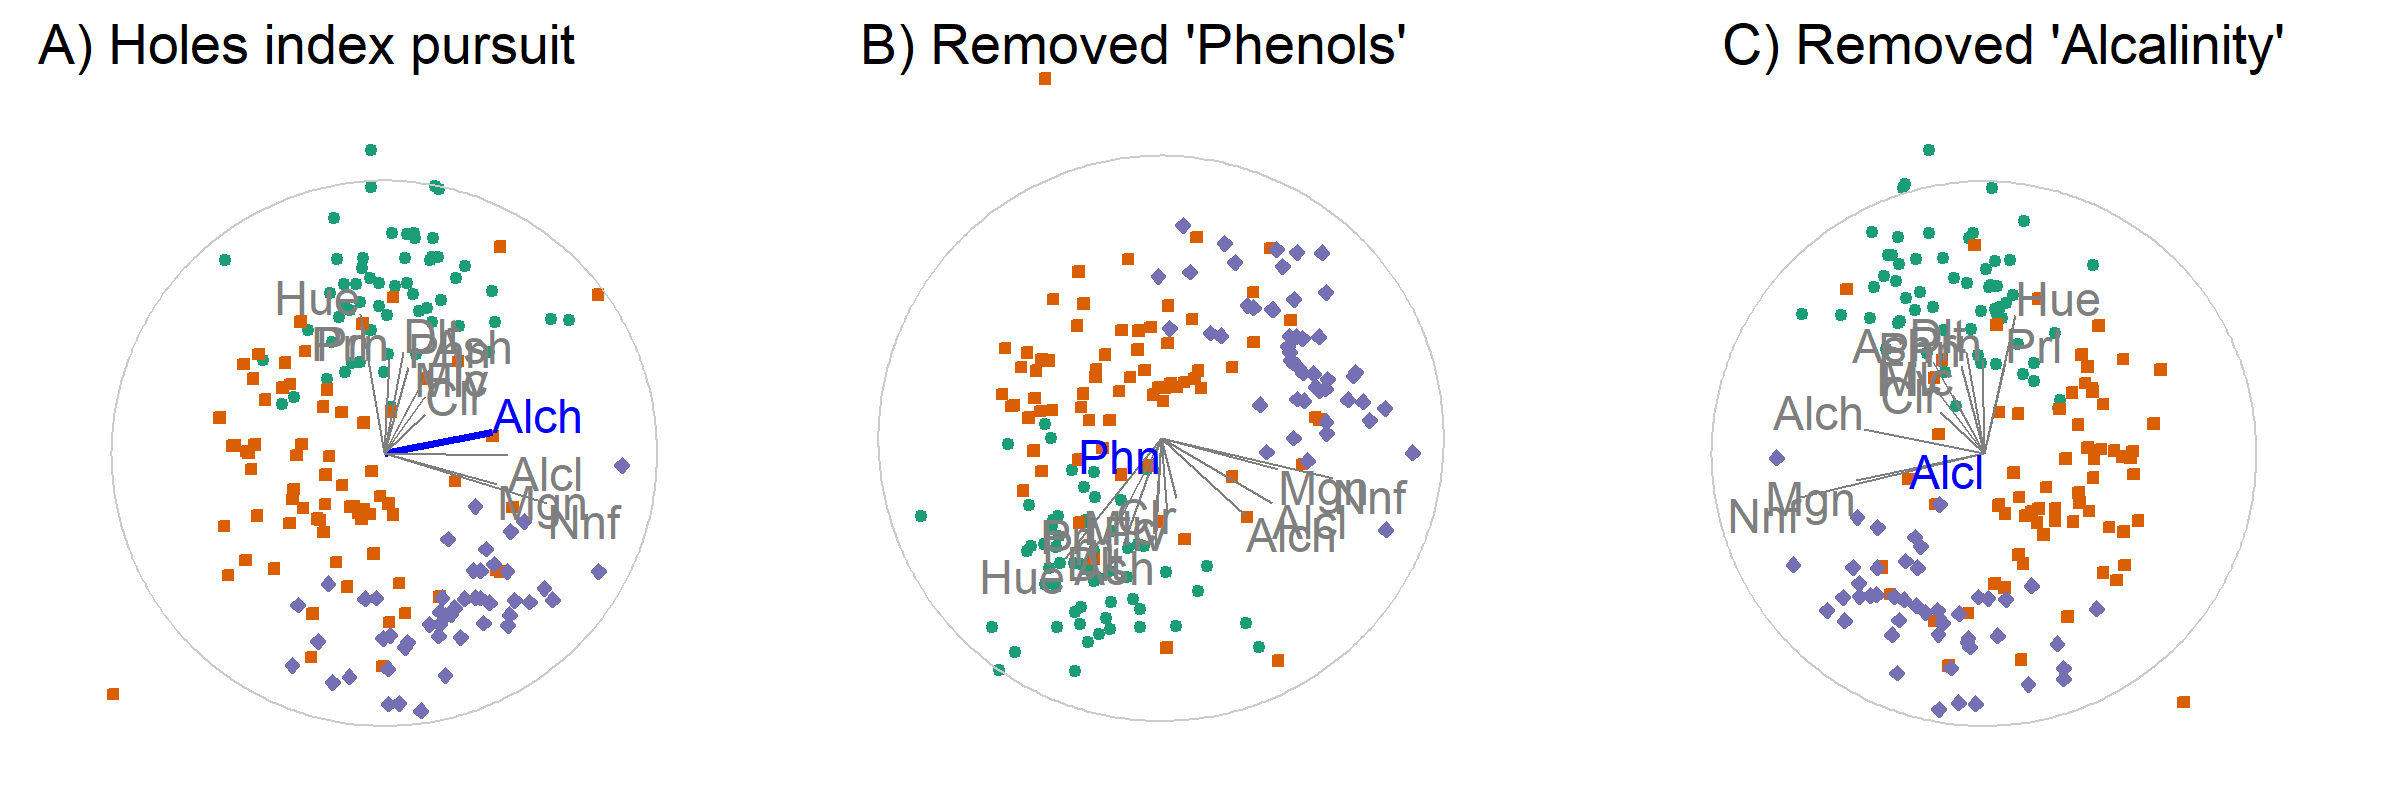
\includegraphics[width=1\linewidth,]{./figures/basisStructureWINE} 

}

\caption{FIXME: CAP NEEDED.}\label{fig:basisStructure}
\end{figure}

\hypertarget{research-objectives}{%
\subsection{Research objectives}\label{research-objectives}}

The overall question of interest is:

\textbf{Can geodesic interpolator with user interaction help analysts understand linear projections of data, and explore the sensitivity of structure in the projection to the variables contributing to the projection?}

which is divided into these more focused objectives:

\begin{enumerate}
\def\labelenumi{\arabic{enumi}.}
\tightlist
\item
  \textbf{How do we define user interaction for a geodesic interpolator to add and remove variables smoothly from a 2D linear projection of data?}\\
  Cook and Buja (1997) described an algorithm for manually controlling a tour (\(p\)-D into 2D), to rotate a variable into and out of a 2D projection. This algorithm provides the start to a human controlled geodesic interpolator (GI). It will be adapted so that the user has more control of the interpolation. The user will be able to set the range of motion from full (-1 to 1) to partial (\(\alpha, \beta\)), to allow the user to intercept the rotation at any step, and to output to a device that allows the user to reproduce motions and animate or rock the rotation backwards and forwards. These fine-tuned controls will provide a better tool for sensitivity analysis.
\end{enumerate}

\begin{enumerate}
\def\labelenumi{\arabic{enumi}.}
\setcounter{enumi}{1}
\item
  \textbf{Do analysts understand the relationship between variables and structure in a 2D linear projection better when the geodesic interpolator is available?}\\
  Current practice for high-dimensional data is to make a single low-dimensional representation, with a method such as principal component analysis (PCA). Often just the first two principal components are shown, which is equivalent to a 2D projection. This technique is also called a biplot. Another more rarely used technique is a tour, which shows an animation of 2D projections. It can be used to get an overview of the structure in the multivariate space, but it is difficult to assess the importance of variables to a particularly interesting low-dimensional structure. A human subject study has been designed and conducted to assess the learning about the importance of variables, from each of these techniques.
\item
  \textbf{Can we define a geodesic interpolator for 3D projections, so that the technology can be implemented in modern virtual reality environments?}\\
  The cutting edge of visualization research today is in virtual environments, as technology has advanced to make this accessible to the masses. It is interesting to explore how analysis with 3D graphics operates in comparison with 2D graphics. Building a GI for 3D projections extends the technology from 2D to 3D, and will allow us to compare the benefits or not, of the new environment for analyzing with multivariate data.
\item
  \textbf{Does 3D provide advantages over 2D, when exploring low-dimensional projections, for understanding structure in high-dimensional data? }\\
  Gracia et al. (2016) compares analyst tasks between 2- and 3-D scatterplots. They find modest accuracy and error improvements for distance perception and outlier identification in favor of 3D at the cost of a relatively small increase in task time. Nelson, Cook, and Cruz-Neira (1998) similarly compare a 2D projection and its 3D manipulation space. They find a slight advantage in the sphere test and a large advantage in the cluster test in favor of the 3D manipulation space. A human subjects experiment will be conducted to assess the sensitivity analysis techniques in a 2D vs 3D environment.
\end{enumerate}

\hypertarget{methodology}{%
\subsection{Methodology}\label{methodology}}

This research is interdisciplinary; touring was developed by statisticians to explore physics data. Modern advances in hardware from information technology allow for 3D rending in higher quality and immersion than previously possible.

The research corresponding with RO \#1 entails \emph{algorithm design} following and further clarifying the work done in Cook and Buja (1997). Adaptations of the algorithm include defining the axis of rotation for manipulation orthogonal to the projection plane. This allowed us to then apply Rodrigues' rotation formula (Rodrigues 1840) to prove the rotation matrix to be used in 2D. We also provide initialization of the in- and out- of plane angles of rotation which clarifies understanding and application of the manual tour.

In the application, attention was given to both pre-compiled tour and human-in-the-loop UCS. We provide an open-source version of the manual tour in the R package, \texttt{spinifex}, which has since been published on CRAN. This forms the foundation for future work in the remaining objectives. In the related paper we additionally apply the algorithm on particle physics data.

For RO \#2 is a controlled \emph{experimental study} to explore the efficacy of interactive UCS compared with the benchmarks factors of PCA and the grand tour. This is designed as a within-participant study where each participant performs all factors. the study is balanced by assigning participants into one of 3 groups where the factor order is controlled by a Latin square while simulation order remains the same. The details are discussed in finer detail in section (\#sec:expStudy), below.

The research for RO \#3 involves \emph{algorithm design} extending the current 2D manual tour into a 3D project. For a 2D projection, the axes basis is rotated through a 3D `manipulation space'. In a 3D projection, such a space requires 4 dimensions. Theoretically, after the addition of a new angle of rotation, the rotation matrix must be extended to accommodate a new dimension and angle parameter. This also means that analysts have another parameter to define, further increasing their already sizable input-volume.

\hypertarget{progress-since-confirmation}{%
\section{Progress since confirmation}\label{progress-since-confirmation}}

During the candidature confirmation review (27 March 2019) we discussed exploratory data analysis, visualization of high dimensional spaces, covered the literature for tours and 3D rendering for information perception. We concluded with the progress for appending the algorithm for the manual tour (RO \# 1), software application in R, and its use on particle physics data.

\hypertarget{published-work}{%
\subsection{Published work}\label{published-work}}

\hypertarget{refereed-journal-article}{%
\subsubsection{Refereed journal article}\label{refereed-journal-article}}

The paper describing the new GI algorithm, the software implementation, and an application, has been published in the R Journal and will appear in the next issue. It is currently available at \href{https://journal.r-project.org/}{journal.r-project.org}.

\hypertarget{software}{%
\subsubsection{Software}\label{software}}

The R package, \texttt{spinifex\ (v0.1.0)} (Spyrison and Cook 2019), has been accepted on the Comprehensive R Archival Network, CRAN (cran.r-project.org/web/packages/spinifex/)(\url{https://cran.r-project.org/web/packages/spinifex/index.html}). A shiny interface was added, which allows analysts to run the GI through a graphical user interface. This will also be used as the experimental apparatus for the experiment to check the effectiveness of the new method.

\hypertarget{sec:expStudy}{%
\subsection{Experimental study}\label{sec:expStudy}}

This study is designed to test the effectiveness of the new GI against current practices: biplot and the grand tour. The design of the experiment is almost finished, and follows these elements. A draft of the working paper is attached with this report.

\hypertarget{sec:factors}{%
\subsubsection{Factors}\label{sec:factors}}

There are three primary factors: principal component analysis (PCA), a grand tour (GT), GI.

\hypertarget{data-structure}{%
\subsubsection{Data structure}\label{data-structure}}

Only one type of data structure will be examined, clusters in multiple dimensions. Data is simulated from a mixture of multivariate normal distributions, with varying cluster means and covariances. Multiple sets of data are simulated, so that each subject will see each data only once. They will see different simulated data from the same model, with the different techniques. Different levels of difficulty are induced by number of variables, number of clusters, and stronger correlation between variables counfounded with clustering. To determine the level of difficulty, distances between clusters means was calculated, and the order of importance of variables was determined by examining the contributions of variables to linear discriminants (Fisher 1936).

\hypertarget{sec:tasks}{%
\subsubsection{Tasks}\label{sec:tasks}}

Participants will perform two tasks, for each factor: identify the number of clusters present in uncoloured data, to check that they understand cluster structure, and secondly, to identify any/all variables that were very important and somewhat important for distinguishing a given cluster from the others, along with reporting the confidence in their answer.

\hypertarget{graphics}{%
\subsubsection{Graphics}\label{graphics}}

The primary display used is a scatterplot. The basis axes projection was also illustrated to the left of the plot. They are shown in a unit circle and show the magnitude and direction each variable contributes to the projection. This is a slight variation in the biplot that will enable users to better read the axes.

\hypertarget{sec:groups}{%
\subsubsection{Groups}\label{sec:groups}}

Each participant will be randomly to one of three groups, setting the order in which the factors are shown. For example, the first group will see PCA, grand tour, and then the GI. Figure \ref{fig:designExample} illustrates the flow of subjects through the experiment.

\begin{figure}[h]

{\centering 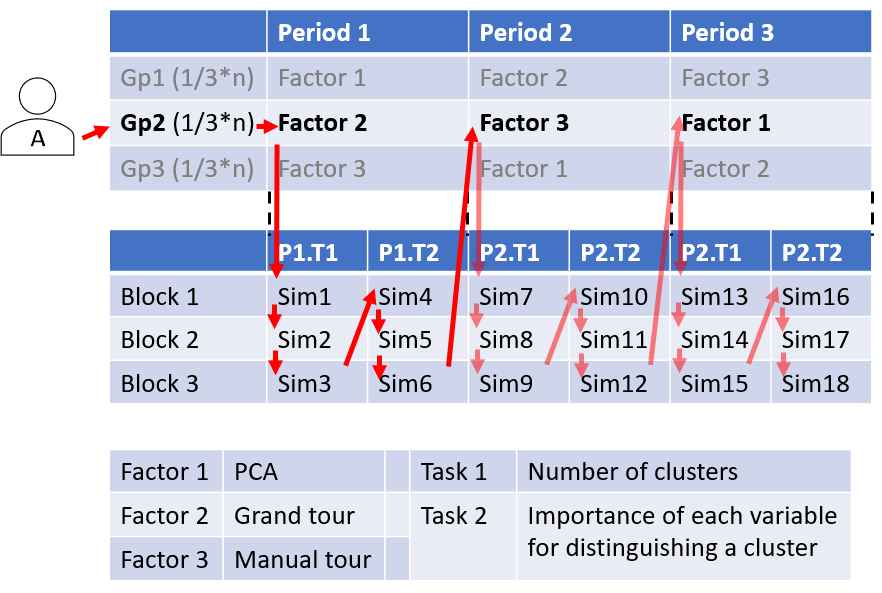
\includegraphics[width=0.8\linewidth,]{./figures/experimental_design_personA} 

}

\caption{Example case. Person 'A' is assigned to group 2, where they will use factor 2 (grand tour) for the first period. They perform 3 block difficulties of task 1 on simulations of increasing difficulty. Then 3 block difficulties of task 2 on unique simulations sampled from the same distributions of increasing difficulty. After this, they proceed to period 2, where they are use factor 3 (manual tour) to perform 3 block difficulties of each task. Lastly, in the third period, they use factor 1 (PCA) to perform the tasks.}\label{fig:designExample}
\end{figure}

\hypertarget{sec:blocks}{%
\subsubsection{Block difficulty}\label{sec:blocks}}

Each participant will do three replications for each factor, one easy, one medium and one difficult.

\hypertarget{experimental-apparatus}{%
\subsubsection{Experimental apparatus}\label{experimental-apparatus}}

A web interface was developed for the experiment. Figure XXX shows the interface for factor 1 (PCA) where the subject is asked how many clusters are present. Figure \ref{fig:basis} shows the interface for factor 3 (GI) where the subject is asked about the impoetance of the variables.

The user interface was consistent across factors, with some slightly differences as required by the different methodology. For example, PCA has 2 radio button inputs selecting principal components to display on the x- and y-axes. The GI had the same axes selection, with the addition of a drop-down bar to select the variable to be controlled and a slider controlling its magnitude.

\begin{figure}[h]

{\centering 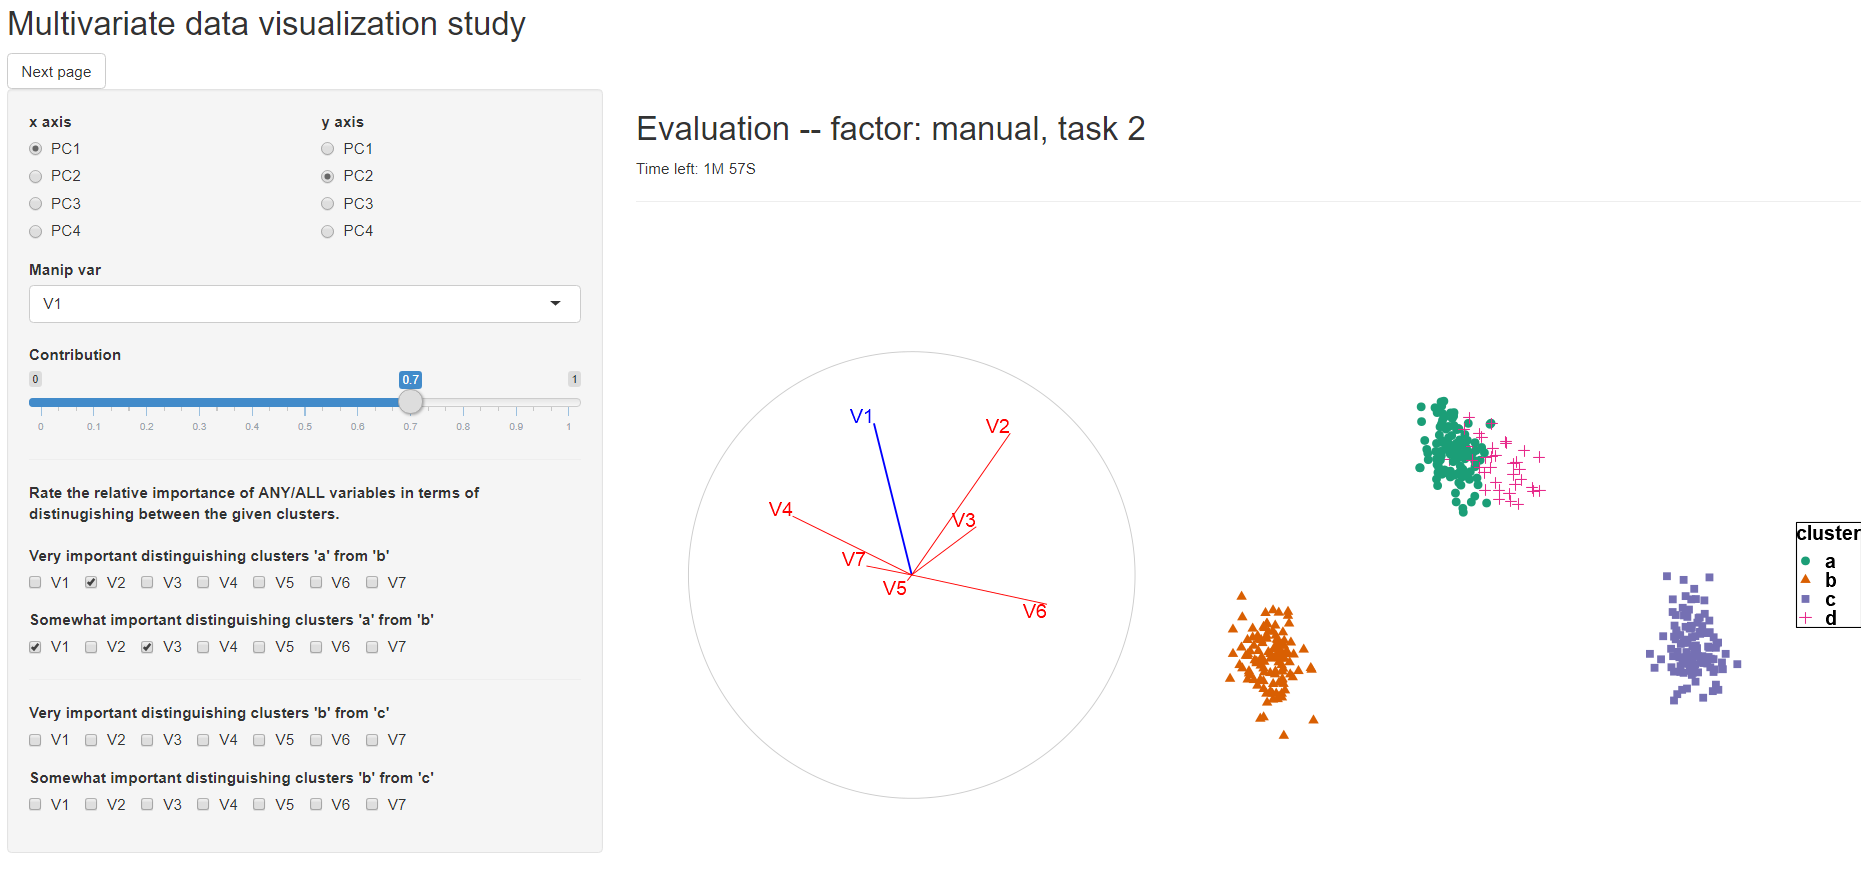
\includegraphics[width=0.8\linewidth,]{./figures/appManualFactor} 

}

\caption{Interface for the manual tour factor in the evaluation section.}\label{fig:appManualFactor}
\end{figure}

Subjects are given two minutes to complete each task, with a timer on the web app indicating time remaining, and their answers are stored in a local file. Demographic information is collected after all tasks are completed, though the web app.

Each subject has an unlimited training time, encouraged to be about 10 minutes, where they watch a video of instructions, and explore the user interfaces.

\hypertarget{pilot-studies}{%
\subsubsection{Pilot studies}\label{pilot-studies}}

Several pilot studies have been conducted, with 4 different people. Each has resulted in improvements to the interface. The data simulation may need to be modified to provide soome clearer distinctions between factors.

\hypertarget{next-steps}{%
\section{Next steps}\label{next-steps}}

\hypertarget{extending-gi-to-3d}{%
\subsection{Extending GI to 3D}\label{extending-gi-to-3d}}

To perform the 2D manual tour, two angle parameters must be identified to perform a rotation of the 3D manipulation space. The angle \(\theta\) indicates the angle on the projection plane between the manipulation variable and the \texttt{x-axis}. While \(\phi\) is the angle that the variable extends into the manipulation space above the projection plane.

A 3D manual tour then must define 3 angle parameters that define the rotation of the 4D manipulation space. Let \(\theta\) now be a set of 2 angles, \(\{\theta_{xy}, \theta_z\}\) that defines the position of the manip variable in the (3D) projection plane and \(\phi\) in the angle it extends into the manipulation direction.

Special care must be taken defining the axis of rotation from the 3D projection into the 4D manipulation space. In particular, the signs will need attention not to be lost especially of trigonometric functions that only support half a rotation. Once this task is done the 4D rotation matrix must be solved, again with the application of Rodrigues' rotation formula (Rodrigues 1840).

\hypertarget{implementation-of-the-3d-gi}{%
\subsection{Implementation of the 3D GI}\label{implementation-of-the-3d-gi}}

In RO \#2, a \texttt{shiny} application was developed and used to explore the effect of user interaction for understanding variable contributions to structure in linear projections. It did so but exploring the differences in performance between 2D biplot of principal components, a 2D grand tour, and a 2D manual tour.

Another R package, \texttt{shinyaframe}, \{Murphy (2017)\} that enables the use of Mozilla's \texttt{aframe} VR product to be consumed in \texttt{shiny} applications. The section titled `Method 2: ``A-Frame and R (Shiny, Ggplot2'')' by Hadjar et al. (2018) is an example of an application with the relevant packages and hardware for display and interaction in stereoscopic virtual reality. This may allow for more rapid advancement in implementation, however, the extent and extendability of interaction remain unknown.

Alternatively, development and application in the game engine Unity would allow for all types of interactions but would likely result in a longer development period.

\hypertarget{proposed-thesis-structure}{%
\section{Proposed thesis structure}\label{proposed-thesis-structure}}

\hypertarget{thesis-structure}{%
\subsection{Thesis structure}\label{thesis-structure}}

This is my assessment of the completion of the thesis research thus far:

\begin{itemize}
\tightlist
\item
  Introduction -- 60\%
\item
  Literature review -- 80\%
\item
  Manual tour and user-controlled steering -- 90\%
\item
  Experimental study -- 60\%
\item
  The extension of the manual tour to 3D -- 0\%
\item
  Conclusion and future plans -- 0\%
\end{itemize}

Figure \ref{fig:timeline} illustrates the purposed timeline for of this research.

\begin{figure}[h]

{\centering 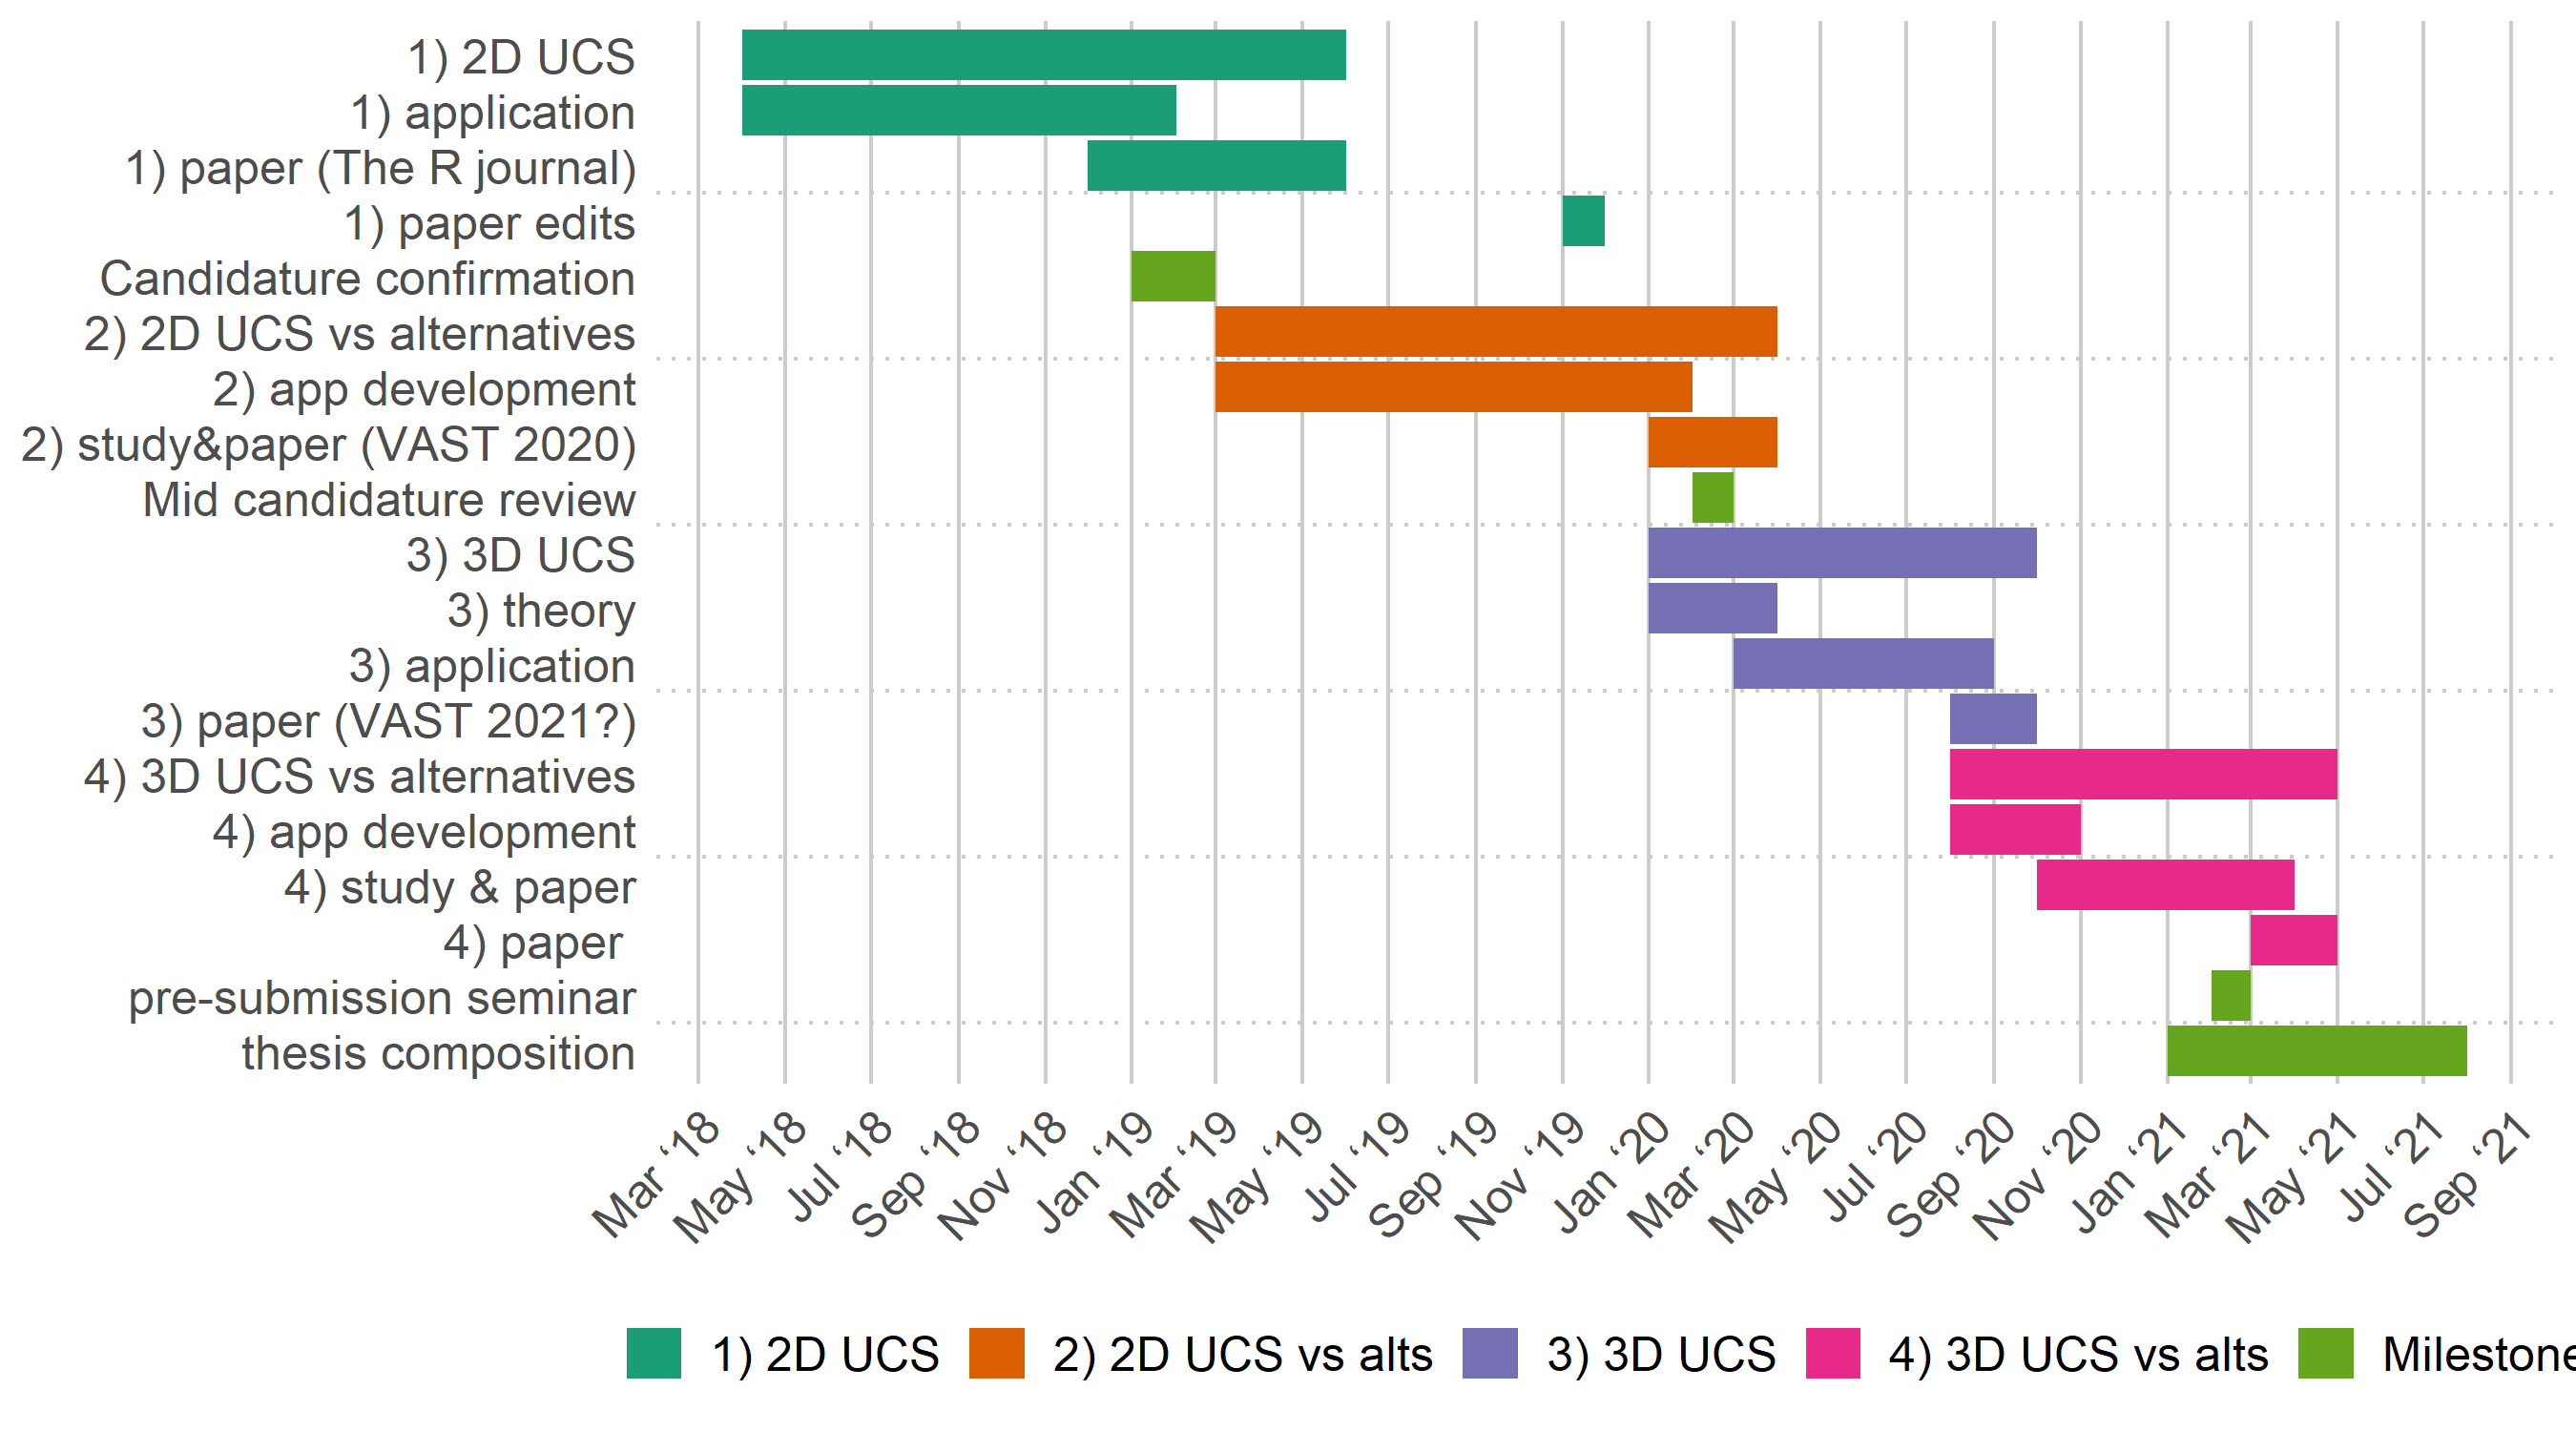
\includegraphics[width=1\linewidth,]{figures/phd_timeline} 

}

\caption{Proposed research timeline.}\label{fig:timeline}
\end{figure}

\hypertarget{program-requirements}{%
\subsection{Program requirements}\label{program-requirements}}

\begin{itemize}
\tightlist
\item
  WES Academic record

  \begin{itemize}
  \tightlist
  \item
    FIT5144: 2019 S1+2, \textbf{In progress}, extended to the pre-submission seminar with the unit coordinator for the usual 2 opportunities to complete.

    \begin{itemize}
    \tightlist
    \item
      Hours: 147\textgreater120 hours \textbf{Tracked}, missing the following requirments (12 hr total)
    \item
      \emph{Needed:} CYR 2 (A \& B) -- 2x 3hr
    \item
      \emph{Needed:} Faculty of IT Workshop 1 and 3 on Ethical Research and Publishing -- 2x 3hr
    \end{itemize}
  \item
    FIT5113: 2018 S2, \textbf{Exemption}
  \item
    FIT6021: 2018 S2, \textbf{Completed} with distinction
  \end{itemize}
\item
  myDevelopment - IT: Monash Doctoral Program - Compulsory Module

  \begin{itemize}
  \tightlist
  \item
    Monash graduate research student induction: \textbf{Completed}
  \item
    Research Integrity - Choose the Option most relevant: \textbf{Completed}
  \item
    Faculty Induction: \textbf{Completed}
  \end{itemize}
\end{itemize}

\hypertarget{potential-issues-for-panel-to-consider}{%
\section{Potential issues for panel to consider}\label{potential-issues-for-panel-to-consider}}

\hypertarget{funding-for-human-subjects}{%
\subsection{Funding for human subjects}\label{funding-for-human-subjects}}

\begin{itemize}
\tightlist
\item
  Beverage voucher: \$6 x 25 people (est) = \$150
\end{itemize}

\hypertarget{support-for-conference-travel}{%
\subsection{Support for conference travel}\label{support-for-conference-travel}}

\textbf{Conferences:}\\
~\\
IEEE VAST 2020: 25-30 October 2020 Salt Lake City, Utah, USA\\
submission: Saturday, March 21, 2020\\
\url{http://ieeevis.org/year/2020/info/call-participation/vast-paper-types}~\\
IEEE VAST 2020: 25-30 October 2020 Salt Lake City, Utah, USA\\
submission: Saturday, March 21, 2020\\

\hypertarget{sec:acknowledgements}{%
\section{Acknowledgements}\label{sec:acknowledgements}}

This report was created in \texttt{R} (R Core Team 2019) using \texttt{rmarkdown} (Xie, Allaire, and Grolemund 2018).

For version control, transparency, and reproducibility, the source files are made available found at \href{https://github.com/nspyrison/mid_candidature}{github.com/nspyrison/mid\_candidature}.

\hypertarget{references}{%
\section*{References}\label{references}}
\addcontentsline{toc}{section}{References}

\hypertarget{refs}{}
\leavevmode\hypertarget{ref-anscombe_graphs_1973}{}%
Anscombe, F. J. 1973. ``Graphs in Statistical Analysis.'' \emph{The American Statistician} 27 (1): 17--21. \url{https://doi.org/10.2307/2682899}.

\leavevmode\hypertarget{ref-cook_manual_1997}{}%
Cook, Dianne, and Andreas Buja. 1997. ``Manual Controls for High-Dimensional Data Projections.'' \emph{Journal of Computational and Graphical Statistics} 6 (4): 464--80. \url{https://doi.org/10.2307/1390747}.

\leavevmode\hypertarget{ref-fisher_use_1936}{}%
Fisher, Ronald A. 1936. ``The Use of Multiple Measurements in Taxonomic Problems.'' \emph{Annals of Eugenics} 7 (2): 179--88. \url{https://doi.org/10.1111/j.1469-1809.1936.tb02137.x}.

\leavevmode\hypertarget{ref-gracia_new_2016}{}%
Gracia, Antonio, Santiago González, Víctor Robles, Ernestina Menasalvas, and Tatiana von Landesberger. 2016. ``New Insights into the Suitability of the Third Dimension for Visualizing Multivariate/Multidimensional Data: A Study Based on Loss of Quality Quantification.'' \emph{Information Visualization} 15 (1): 3--30. \url{https://doi.org/10.1177/1473871614556393}.

\leavevmode\hypertarget{ref-hadjar_webvr_2018}{}%
Hadjar, Hayet, Abdelkrim Meziane, Rachid Gherbi, Insaf Setitra, and Noureddine Aouaa. 2018. ``WebVR Based Interactive Visualization of Open Health Data.'' In \emph{Proceedings of the 2nd International Conference on Web Studies}, 56--63.

\leavevmode\hypertarget{ref-kruskal_toward_1969}{}%
Kruskal, Joseph B. 1969. ``Toward a Practical Method Which Helps Uncover the Structure of a Set of Multivariate Observations by Finding the Linear Transformation Which Optimizes a New `Index of Condensation'.'' In \emph{Statistical Computation}, edited by Roy C. Milton and John A. Nelder, 427--40. Academic Press. \url{https://doi.org/10.1016/B978-0-12-498150-8.50024-0}.

\leavevmode\hypertarget{ref-matejka_same_2017}{}%
Matejka, Justin, and George Fitzmaurice. 2017. ``Same Stats, Different Graphs: Generating Datasets with Varied Appearance and Identical Statistics Through Simulated Annealing.'' In \emph{Proceedings of the 2017 CHI Conference on Human Factors in Computing Systems - CHI '17}, 1290--4. Denver, Colorado, USA: ACM Press. \url{https://doi.org/10.1145/3025453.3025912}.

\leavevmode\hypertarget{ref-murphy_shinyaframe_2017}{}%
Murphy, William. 2017. \emph{Shinyaframe: 'WebVR' Data Visualizations with 'RStudio Shiny' and 'Mozilla a-Frame'} (version R package version 1.0.1). \url{https://CRAN.R-project.org/package=shinyaframe}.

\leavevmode\hypertarget{ref-nelson_xgobi_1998}{}%
Nelson, Laura, Dianne Cook, and Carolina Cruz-Neira. 1998. ``XGobi Vs the C2: Results of an Experiment Comparing Data Visualization in a 3-d Immer- Sive Virtual Reality Environment with a 2-d Workstation Display.'' \emph{Computational Statistics} 14 (1): 39--52.

\leavevmode\hypertarget{ref-pearson_liii._1901}{}%
Pearson, Karl. 1901. ``LIII. On Lines and Planes of Closest Fit to Systems of Points in Space.'' \emph{The London, Edinburgh, and Dublin Philosophical Magazine and Journal of Science} 2 (11): 559--72.

\leavevmode\hypertarget{ref-r_core_team_r:_2019}{}%
R Core Team. 2019. \emph{R: A Language and Environment for Statistical Computing}. Vienna, Austria: R Foundation for Statistical Computing. \url{https://www.R-project.org/}.

\leavevmode\hypertarget{ref-rodrigues_lois_1840}{}%
Rodrigues, Olinde. 1840. \emph{Des Lois Géométriques Qui Régissent Les Déplacements d'un Système Solide Dans L'espace: Et de La Variation Des Cordonnées Provenant de Ces Déplacements Considérés Indépendamment Des Causes Qui Peuvent Les Produire}.

\leavevmode\hypertarget{ref-spyrison_spinifex_2019}{}%
Spyrison, Nicholas S., and Dianne Cook. 2019. \emph{Spinifex: Manual Tours, Manual Control of Dynamic Projections of Numeric Multivariate Data} (version 0.1.0.9000). \url{https://github.com/nspyrison/spinifex/}.

\leavevmode\hypertarget{ref-tukey_exploratory_1977}{}%
Tukey, John W. 1977. \emph{Exploratory Data Analysis}. Vol. 32. Pearson.

\leavevmode\hypertarget{ref-wickham_tourr:_2011}{}%
Wickham, Hadley, Dianne Cook, Heike Hofmann, and Andreas Buja. 2011. ``Tourr: An R Package for Exploring Multivariate Data with Projections.'' \emph{Journal of Statistical Software} 40 (2). \url{https://doi.org/10.18637/jss.v040.i02}.

\leavevmode\hypertarget{ref-xie_r_2018}{}%
Xie, Yihui, J. J. Allaire, and Garrett Grolemund. 2018. \emph{R Markdown: The Definitive Guide}. Boca Raton, Florida: Chapman; Hall/CRC. \url{https://bookdown.org/yihui/rmarkdown}.


\end{document}
